
\documentclass{standalone}
\usepackage[svgnames]{xcolor}
\usepackage{pgfplots}
\pgfplotsset{compat=newest}
\usepackage[sfdefault]{FiraSans}
\usepackage{FiraMono}
\renewcommand*\familydefault{\sfdefault}
\begin{document}
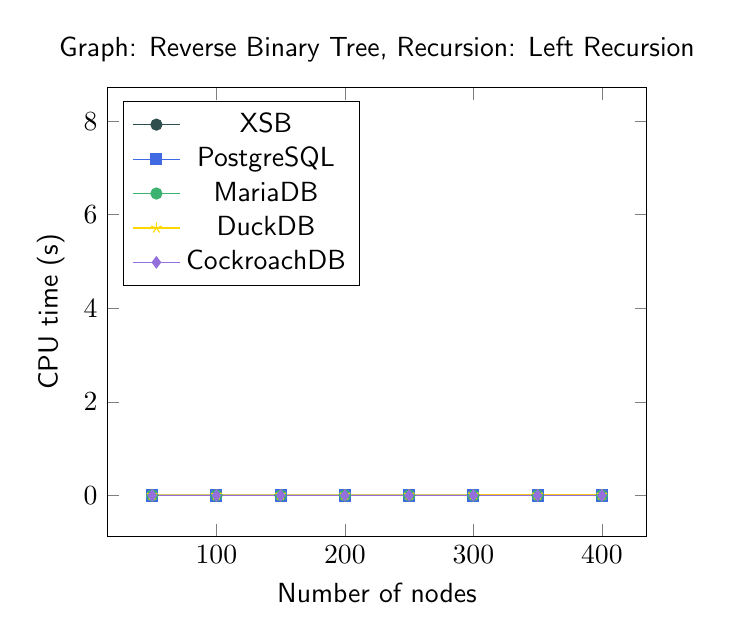
\begin{tikzpicture}
    \begin{axis}[
        title={Graph: Reverse Binary Tree, Recursion: Left Recursion},
        xlabel={Number of nodes},
        ylabel={CPU time (s)},
        legend pos={north west},
        ymax=8.712522
    ]
    \addplot+[DarkSlateGray, mark options={color=DarkSlateGray}] coordinates {(50,4.000000000000185e-05) (100,7.299999999999665e-05) (200,0.00011349999999999896) (250,0.000137500000000002) (150,0.000174000000000001) (400,0.000298) (300,0.0003435) (350,0.000445499999999998)};
\addlegendentry{XSB}
\addplot+[RoyalBlue, mark options={color=RoyalBlue}] coordinates {(50,0.00011264999999999192) (200,0.00011279999999999624) (150,0.0001131500000000063) (250,0.00011549999999999061) (400,0.0001244999999999996) (350,0.0001285000000000036) (300,0.00013410000000002587) (100,0.00019114999999997329)};
\addlegendentry{PostgreSQL}
\addplot+[MediumSeaGreen, mark options={color=MediumSeaGreen}] coordinates {(250,0.00011905000000000943) (50,0.00012139999999999374) (100,0.00013075000000004056) (150,0.00013120000000002574) (350,0.00013189999999999036) (300,0.0001376999999999906) (400,0.00014039999999998498) (200,0.0001528999999999836)};
\addlegendentry{MariaDB}
\addplot+[Gold, mark options={color=Gold}] coordinates {(50,0.008513949999999992) (100,0.01098685000000002) (250,0.011777999999999983) (150,0.012931600000000015) (200,0.012960449999999984) (400,0.014136250000000045) (350,0.015241849999999973) (300,0.017736949999999974)};
\addlegendentry{DuckDB}
\addplot+[MediumPurple, mark options={color=MediumPurple}] coordinates {(350,0.0001589499999999633) (300,0.00017924999999999192) (100,0.00018764999999998366) (250,0.00019859999999996547) (50,0.00020100000000006224) (150,0.0002027000000000001) (400,0.00020625000000001892) (200,0.00024299999999999322)};
\addlegendentry{CockroachDB}

    \end{axis}
\end{tikzpicture}
\end{document}
